% \begin{document}

\usetikzlibrary{arrows.meta} % For double arrows

\chapter{Dropbox}

TLA+ is a \textit{thinking tool}. Writing a specification with TLA+ and verify
it against the model checker encourages the designer to exhaustively consider
all corner cases in the design. In this chapter, we will specify a Dropbox-like
service with TLA+ and use the model checker to flesh out the design.\\

\section{Design}

The simplified Dropbox-like service includes a block server that holds physical 
copies of all versions of user files, and a meta server that holds meta data on
all the files and path to the block server. A client contacts both meta and
block server as needed to keep up-to-date. In this design, client attempts to
stay up-to-date on all the file meta, but selectively download the physical
files as needed to save bandwidth.\\

A client can make local changes to a file. The updated file is committed when
the client syncs with meta and block server. The change is then propagated to
the other clients. If multiple clients made changes to the same file, the first
one to upload wins and the other clients need to rebase their changes on top of
latest and attempt to upload again.\\

The system design is visualized below:\\

\begin{center}
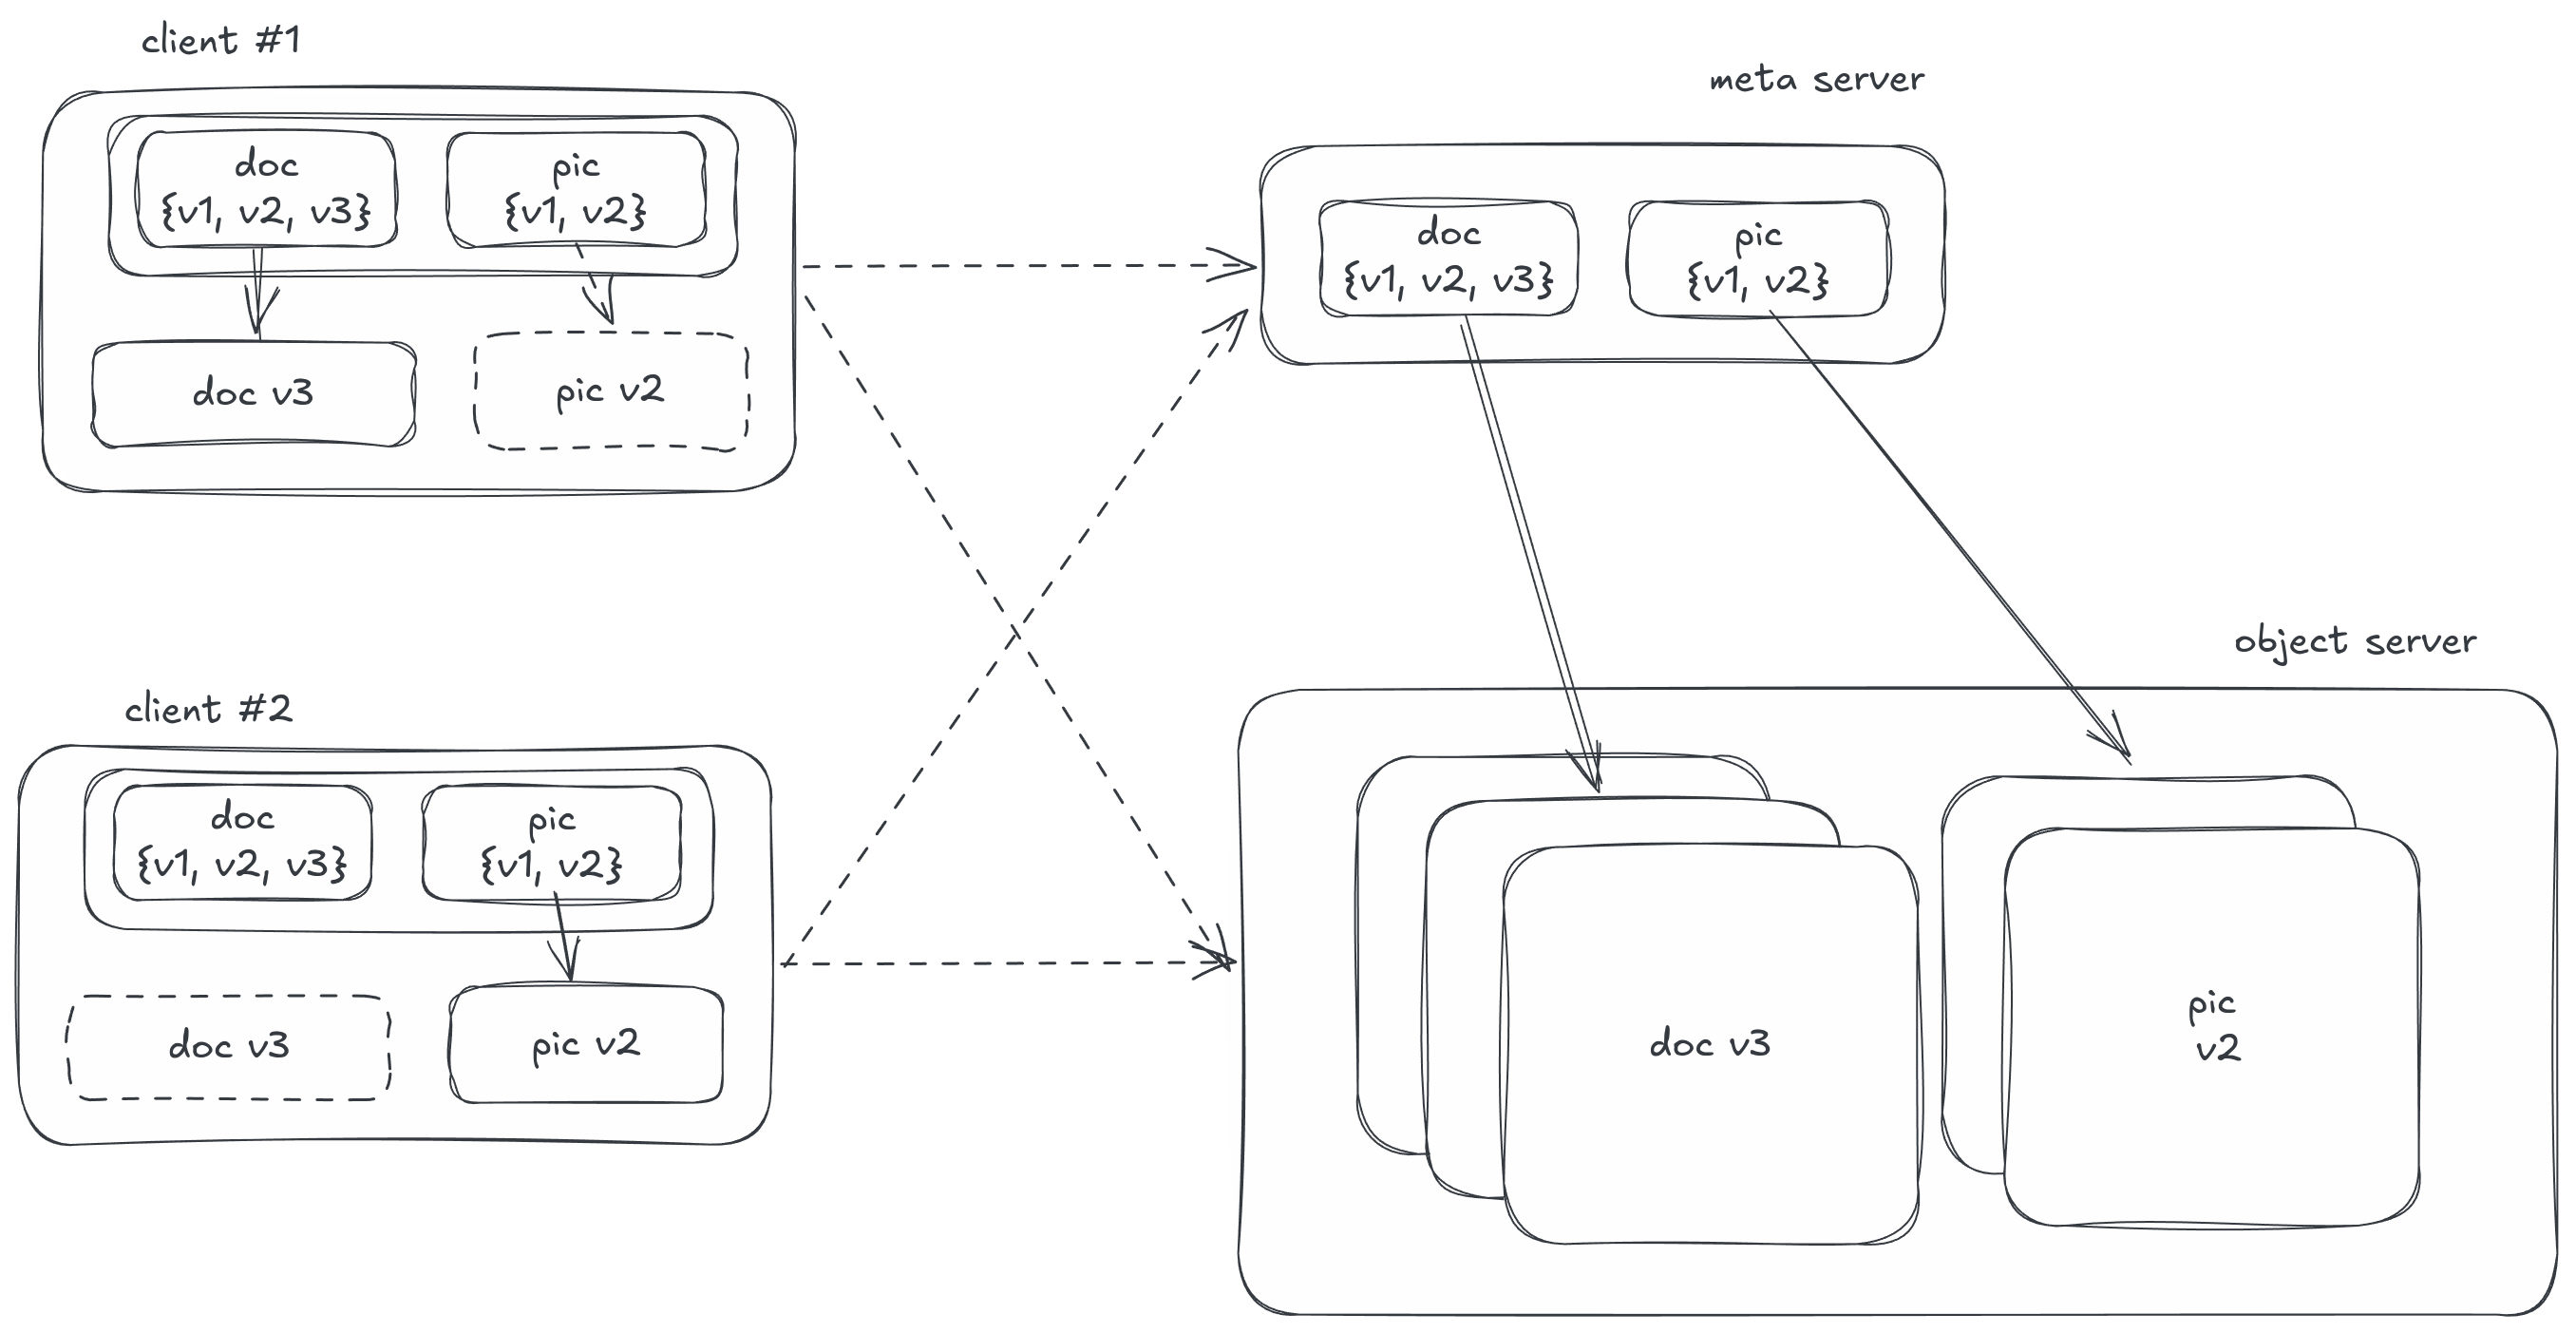
\includegraphics[width=300pt]{dropbox}
\end{center}

\section{Spec}

The core set of actions is defined below:\\
\begin{tla}
Next ==
    \/ \E k \in Clients: 
        \E f \in Files: 
            \/ SyncMeta(k, f)
            \/ Download(k, f)
            \/ Modify(k, f)
            \/ Upload(k, f)
\end{tla}
\begin{tlatex}
\@x{ Next \.{\defeq}}%
\@x{\@s{16.4} \.{\lor} \E\, k \.{\in} Clients \.{:}}%
\@x{\@s{20.5} \E\, f \.{\in} Files \.{:}}%
\@x{\@s{24.6} \.{\lor} SyncMeta ( k ,\, f )}%
\@x{\@s{24.6} \.{\lor} Download ( k ,\, f )}%
\@x{\@s{24.6} \.{\lor} Modify ( k ,\, f )}%
\@x{\@s{24.6} \.{\lor} Upload ( k ,\, f )}%
\end{tlatex}
\\

In every state, the system can choose to synchronize file meta, download a file,
modify a file, or upload a file. Some of these operations depend on each other.
For example, a file can only be modified if it has been downloaded.\\ 

The following describes the variables used track system state:\\
\begin{tla}
Init ==
    /\ meta_server = [f \in Files |-> {1}]
    /\ block_server = [f \in Files |-> {1}]
    /\ client_meta = [k \in Clients |-> [f \in Files |-> {1}]]
    /\ client_block = [k \in Clients |-> <<>>]
\end{tla}
\begin{tlatex}
\@x{ Init \.{\defeq}}%
 \@x{\@s{16.4} \.{\land} meta\_server \.{=} [ f \.{\in} Files \.{\mapsto} \{ 1
 \} ]}%
 \@x{\@s{16.4} \.{\land} block\_server \.{=} [ f \.{\in} Files \.{\mapsto} \{
 1 \} ]}%
 \@x{\@s{16.4} \.{\land} client\_meta \.{=} [ k \.{\in} Clients \.{\mapsto} [
 f \.{\in} Files \.{\mapsto} \{ 1 \} ] ]}%
 \@x{\@s{16.4} \.{\land} client\_block \.{=} [ k \.{\in} Clients \.{\mapsto}
 {\langle} {\rangle} ]}%
\end{tlatex}\\

\begin{itemize}
    \item \textit{meta\_server} is a lookup table from filename to a set of revisions.
    \item \textit{block\_server} is a lookup table from filename to a set of revisions.
    \item \textit{client\_meta} represents client's meta.
    \item \textit{client\_block} is client's block storage, only holding one version of the file. 
\end{itemize}

\section{Safety}

\section{Liveness}

% \end{document}

